\documentclass[a4paper, 11pt]{article}

% Nécessaire
\usepackage[french]{babel}
\usepackage[utf8]{inputenc}
\usepackage[T1]{fontenc}
\usepackage{lmodern}
\usepackage{amsmath, amsthm}
\usepackage{amsfonts,amssymb}

% Marge
\usepackage{geometry}
\geometry{margin={2.1cm ,2.1cm}}

% Figures, graphiques
\usepackage{graphicx}
\usepackage{epsfig}
\usepackage{caption}

% Surlignage
\usepackage{alltt}

\usepackage{xcolor}
\usepackage{soul}
\usepackage{color}
\usepackage{colortbl}

% Indicatrice
\usepackage{dsfont}

\usepackage{multirow}
\usepackage{eurosym}
\usepackage{extarrows}


% Titre
\title{Effets des paramètres fixes sur le modèle}
\author{}
\date{}
 
\begin{document}
 
\maketitle
 
Ce document à pour but de montrer les effets des paramètres fixes sur le modèle. Lesdits paramètres fixes sont recensés dans le tableau qui suit avec leur valeur par défaut.
\begin{center}
\begin{tabular}{lll}
\textbf{Paramètre} & \textbf{Notation} & \textbf{Valeur par défaut}\\
\textit{Sex-ratio} & $SR$ & 0.5\\
Proba de survie au paillage synthétique & $\mu_{PS}$ & 0\\
Proba d'entrer en pupaison & $p_{pup}$ & 0.77\\
Durée de pupaison & $d_p$ & 5\\
Nombres d'oeufs pondus / femelles & E & 150\\
Proba de survie des oeufs & $\mu$ & 0.04
\end{tabular}
\end{center}

\section{Référence}

Pour mieux illuster l'effet de chaque paramètres, on se servira d'une courbe de référence qui utilisera les valeurs par défaut.

\begin{figure}[h]
 \centering
 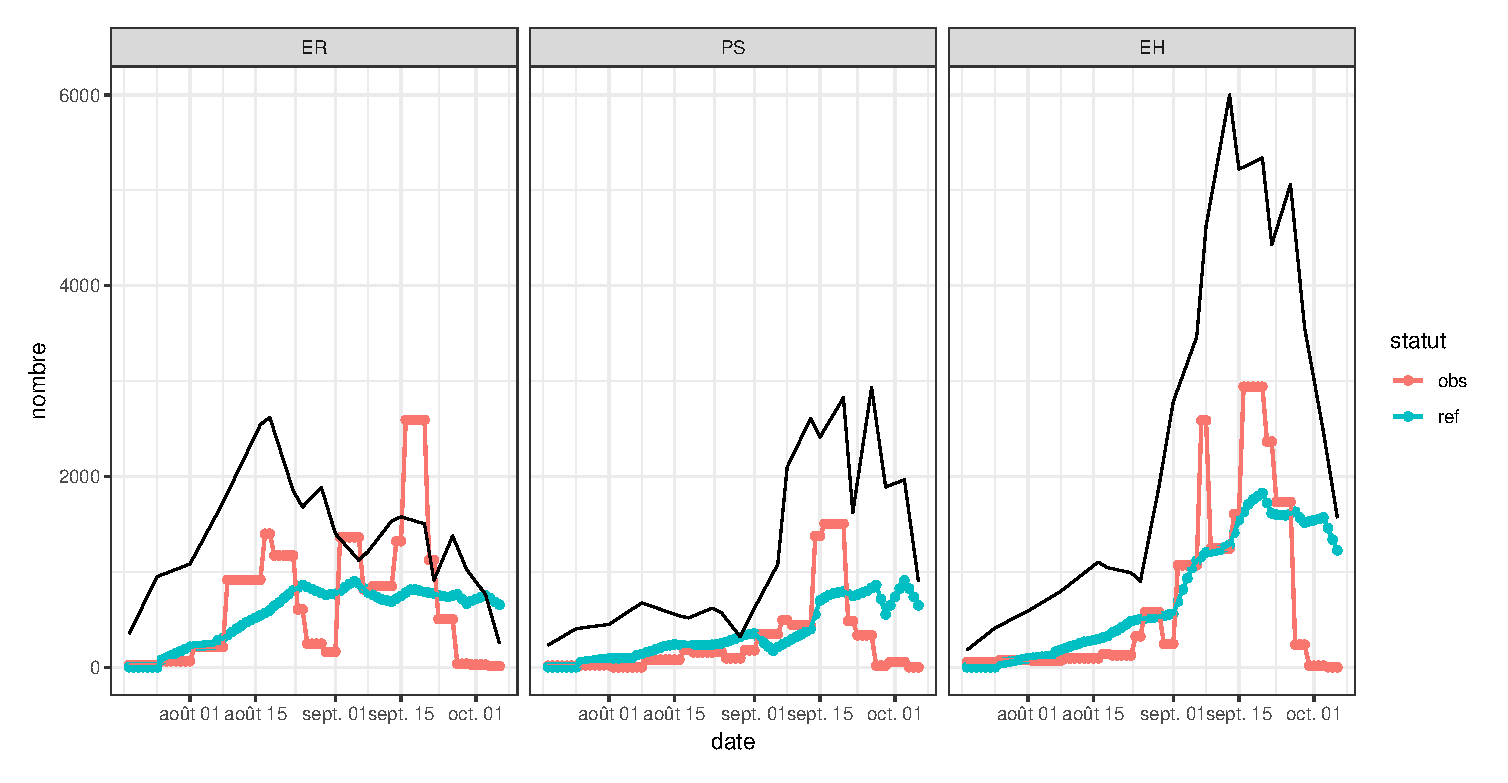
\epsfig{file = plots/ref_inflos.eps, scale = 0.65}
 \caption{Comparaison des larves observées et estimées. En noir sont visibles les inflorescences.}
\end{figure}

Les paramètres calibrés sont ici égaux à 

\begin{center}
\begin{tabular}{lllll}
$\gamma$ & $p_m$ & $\mu_{ER}$ & $\mu_{EH}$ & $k$\\
0.04 & 0.58 & 0.52 & 0 & 6.91
\end{tabular}
\end{center}


\newpage
\section{Les œufs}
 
Le premier paramètre auquel on s'intéresse est le nombre d'œufs pondus par une femelle.
On commence par fixer le paramètre à $E = 450$. Et on obtient

\begin{figure}[h]
 \centering
 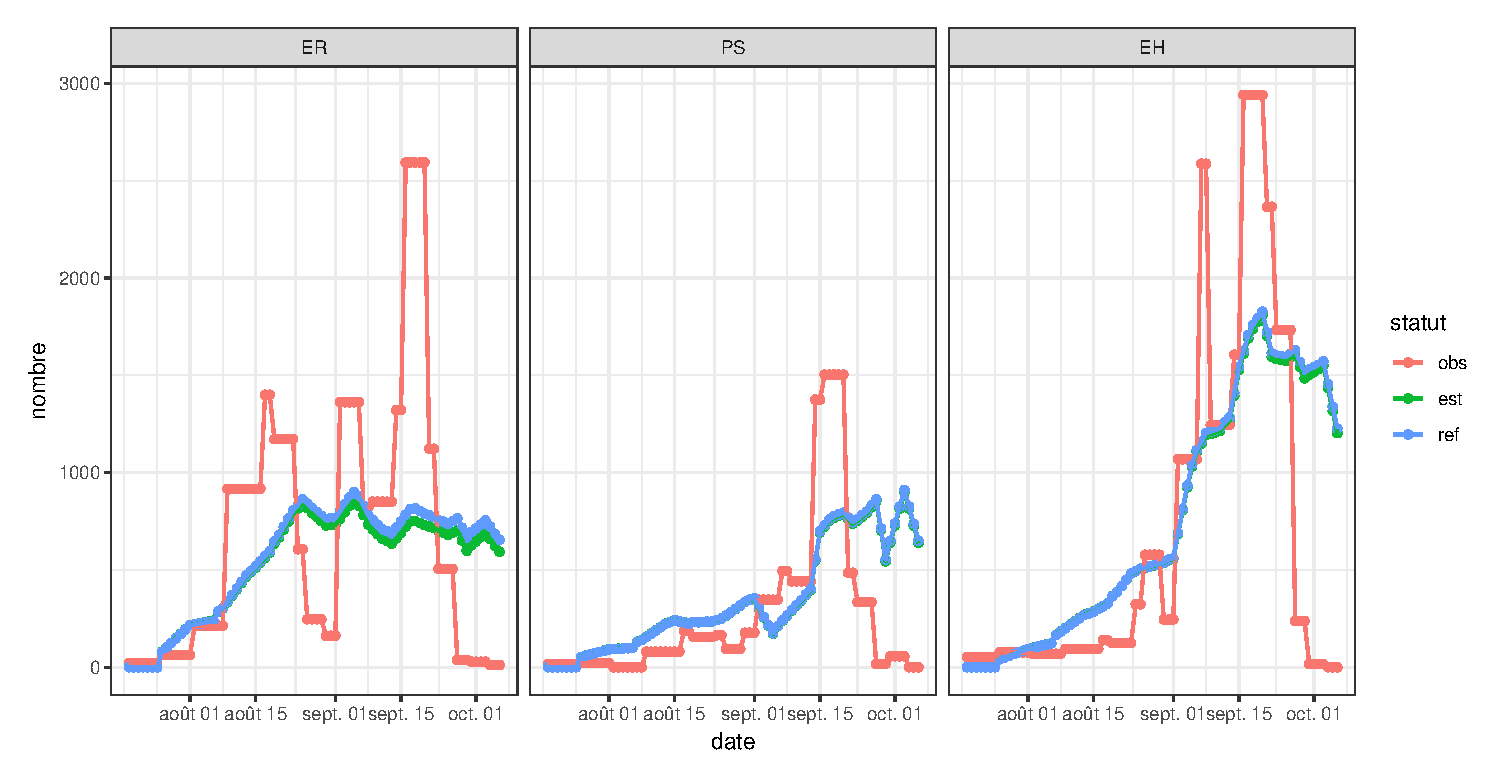
\epsfig{file = plots/eggs450.eps, scale = 0.65}
 \caption{Comparaison des larves observées et estimées. En bleu est visible l'estimation de référence.}
\end{figure}

Les paramètres calibrés sont ici égaux à 

\begin{center}
\begin{tabular}{lllll}
$\gamma$ & $p_m$ & $\mu_{ER}$ & $\mu_{EH}$ & $k$\\
0.01 & 0.62 & 0.19 & 0 & 49.4
\end{tabular}
\end{center}

Avec $E = 50$ : 

\begin{figure}[h]
 \centering
 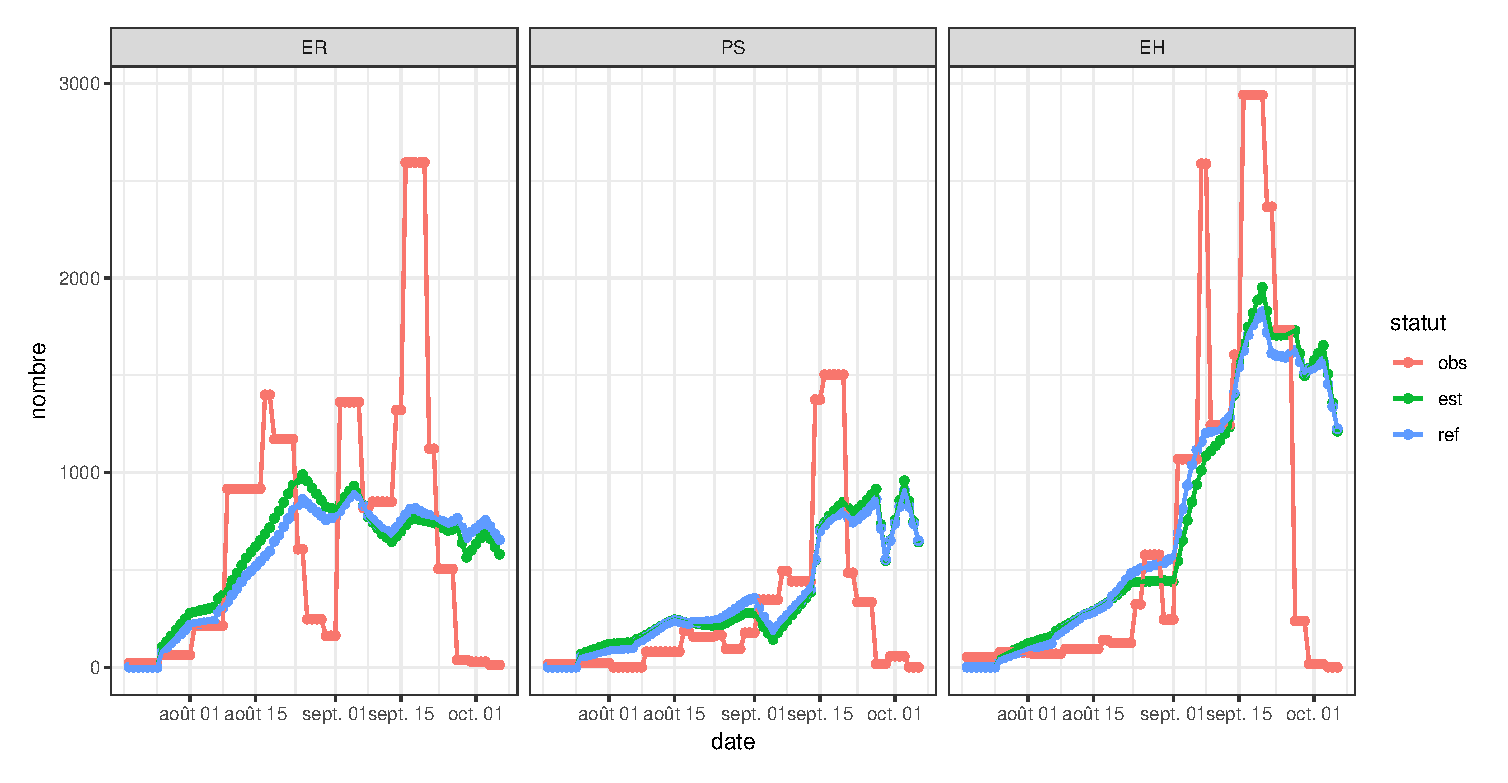
\epsfig{file = plots/eggs50.eps, scale = 0.65}
 \caption{Comparaison des larves observées et estimées. En bleu est visible l'estimation de référence.}
\end{figure}

Les paramètres calibrés sont ici égaux à 

\begin{center}
\begin{tabular}{lllll}
$\gamma$ & $p_m$ & $\mu_{ER}$ & $\mu_{EH}$ & $k$\\
0.24 & 0.47 & 0.96 & 0 & 38.6
\end{tabular}
\end{center}


Une autre tentative a été effectuée. Les individus exogènes arrivent non plus proportionnellement au nombre d'inflorescences, mais au nombre de 20 chaque jour. Le nombre d'œufs a été fixé à 300. Voici les résultats :

\begin{figure}[h]
 \centering
 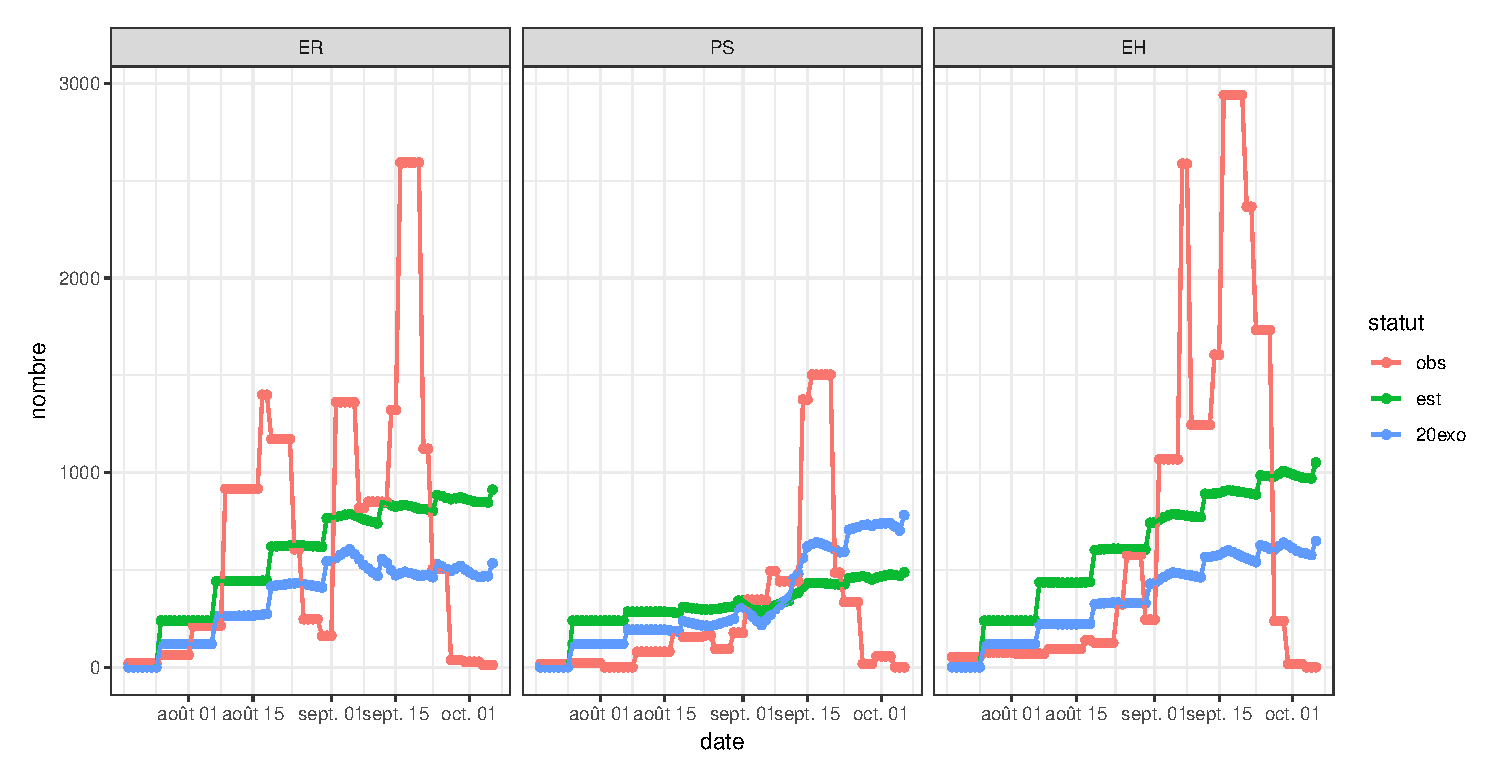
\epsfig{file = plots/eggs300.eps, scale = 0.65}
 \caption{Comparaison des larves observées et estimées. En bleu est visible l'estimation avec des exogènes $=20$.}
\end{figure}

Les paramètres calibrés sont ici égaux à 

\begin{center}
\begin{tabular}{llll}
 $p_m$ & $\mu_{ER}$ & $\mu_{EH}$ & $k$\\
0.7 & 0.28 & 0.86 & 36.7
\end{tabular}
\end{center}

pour la référence et à 

\begin{center}
\begin{tabular}{llll}
 $p_m$ & $\mu_{ER}$ & $\mu_{EH}$ & $k$\\
0.28 & 0.0.19 & 0.2 & 49.4
\end{tabular}
\end{center}

pour l'estimation avec $E = 300$.
Ci-dessous un graphique pour illuster la valeur que prend $\gamma$ en fonction du $E$ fixé.

\begin{figure}[h]
 \centering
 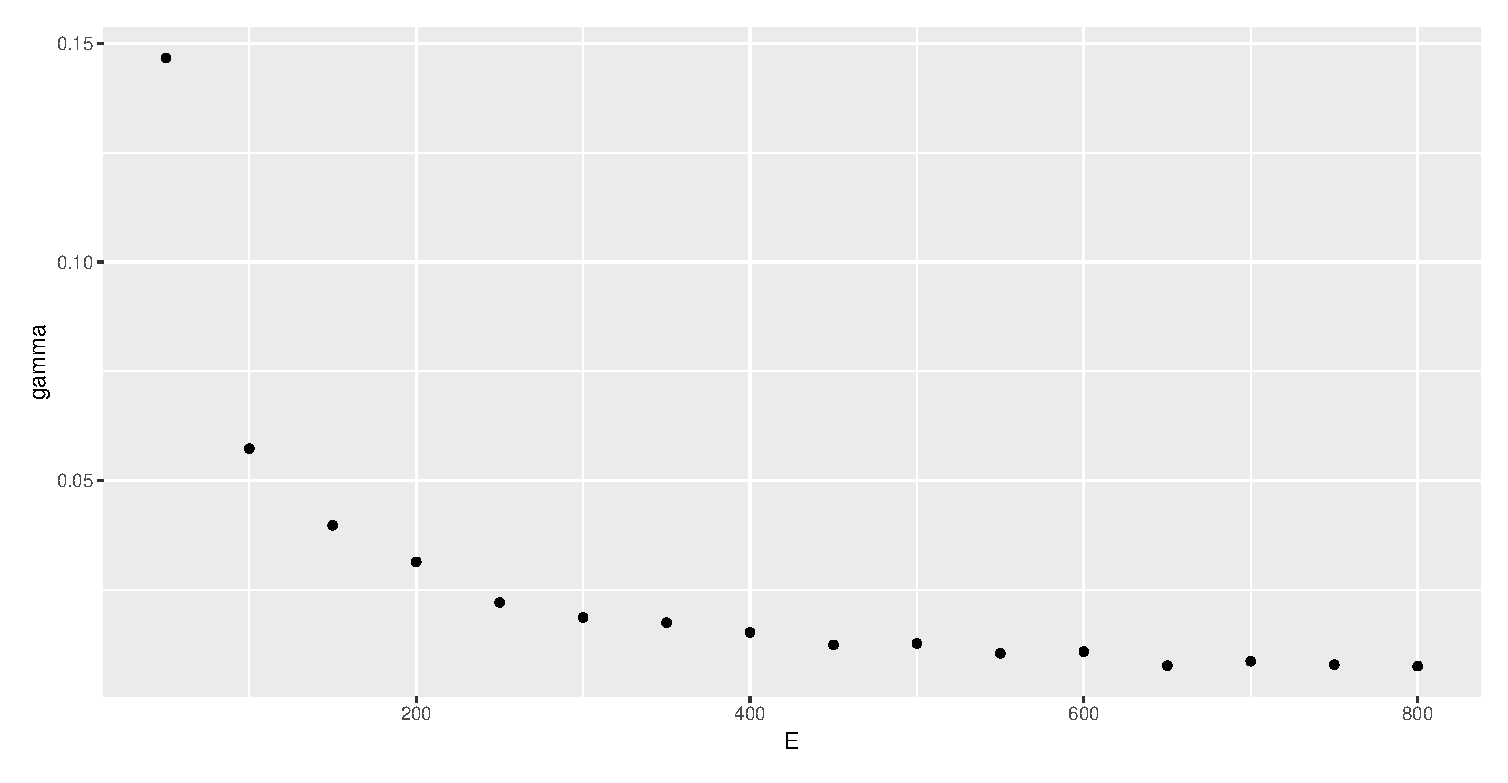
\epsfig{file = plots/gamma_V_eggs.eps, scale = 0.5}
 \caption{$\gamma$ en fonction de $E$.}
\end{figure}

\newpage
\section{Proba d'entrer en pupaison}

La valeur par défaut de $p_pup$ est 0.77. Essayons $p_{pup} = 1$ :

\begin{figure}[h]
 \centering
 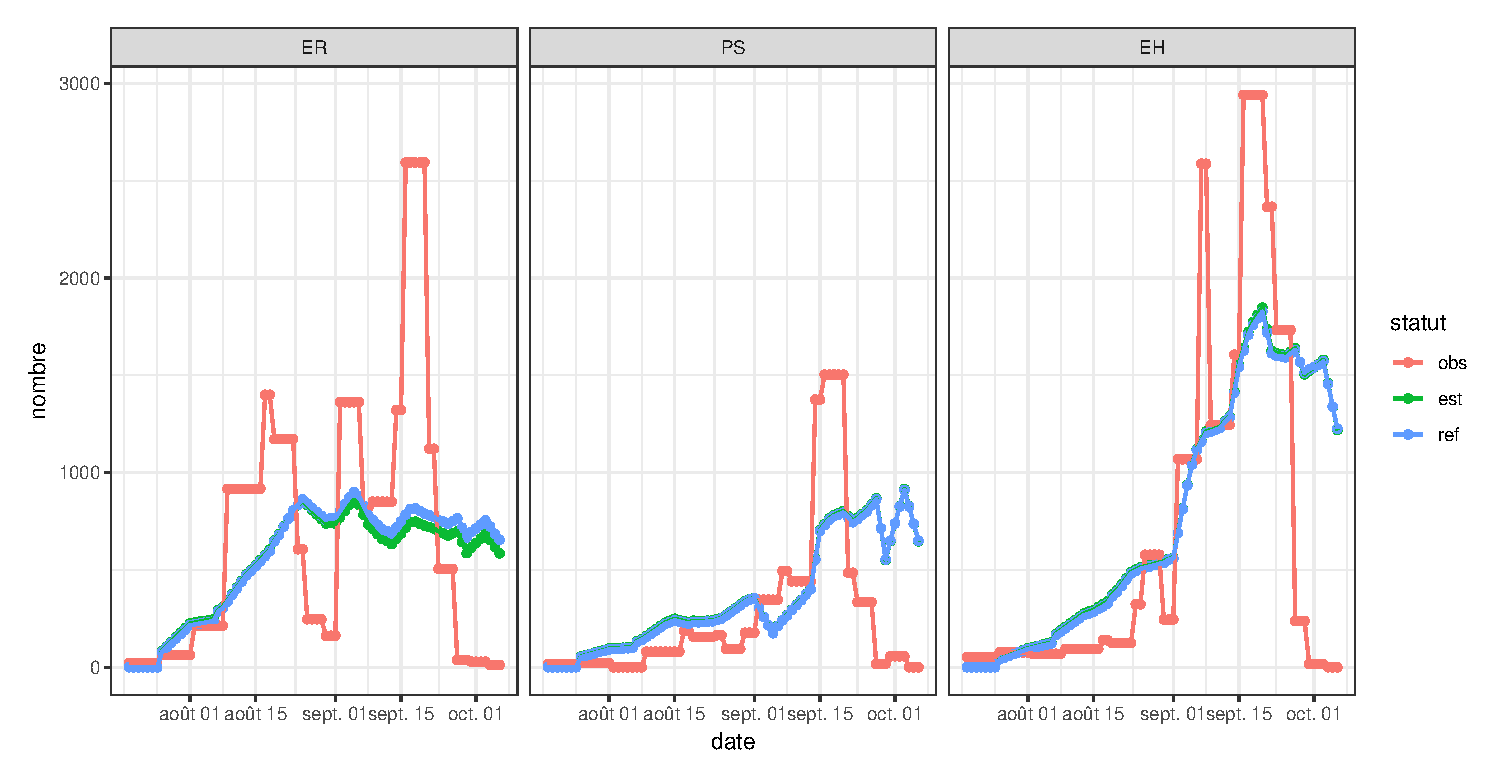
\epsfig{file = plots/pupe_1.eps, scale = 0.65}
 \caption{Comparaison des larves observées et estimées. En bleu est visible l'estimation de référence.}
\end{figure}

Les paramètres calibrés sont ici égaux à 

\begin{center}
\begin{tabular}{lllll}
$\gamma$ & $p_m$ & $\mu_{ER}$ & $\mu_{EH}$ & $k$\\
0.034 & 0.65 & 0.54 & 0 & 12.5
\end{tabular}
\end{center}


Avec $p_{pup} = 0.4$ : 


\begin{figure}[h]
 \centering
 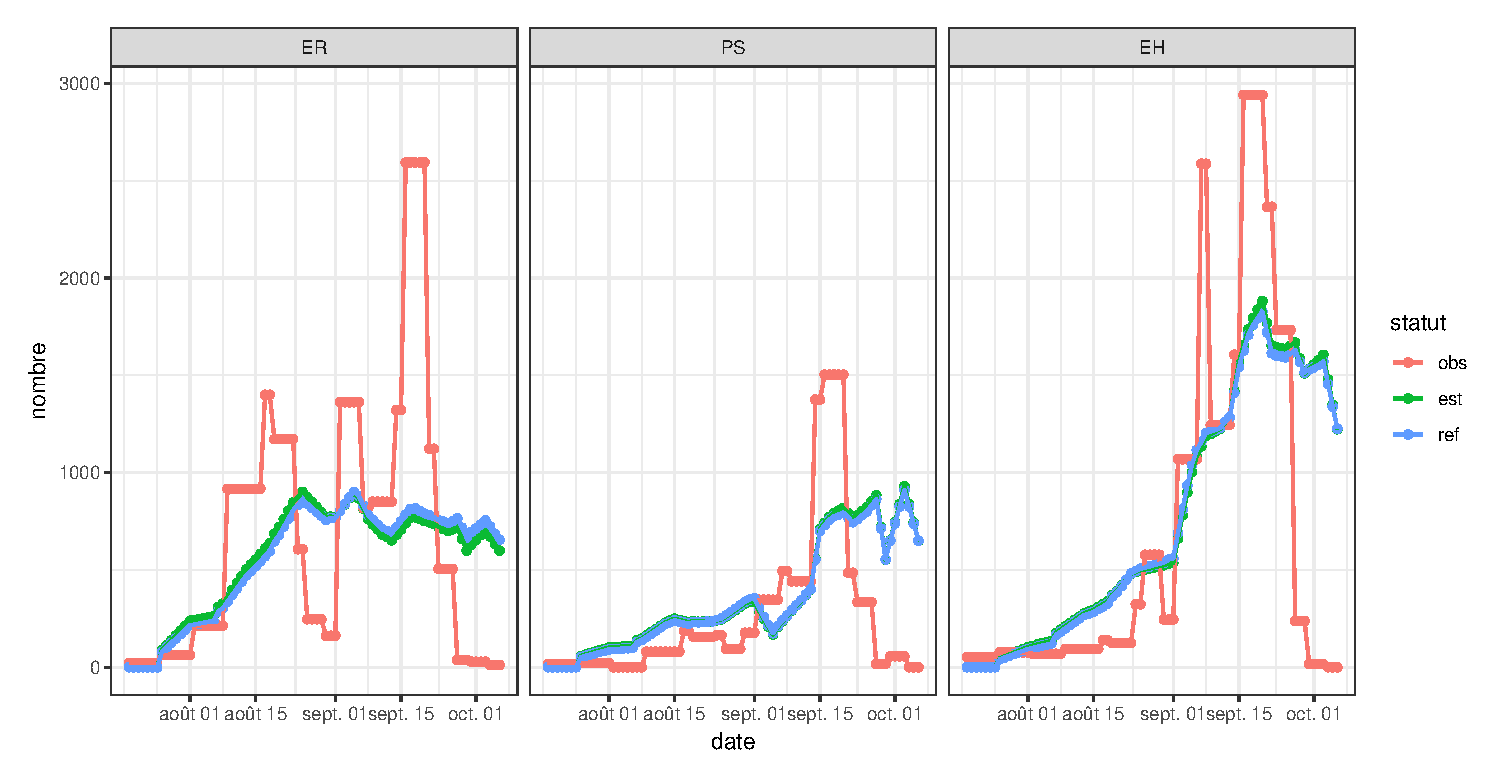
\epsfig{file = plots/pupe_04.eps, scale = 0.65}
 \caption{Comparaison des larves observées et estimées. En bleu est visible l'estimation de référence.}
\end{figure}

Les paramètres calibrés sont ici égaux à 

\begin{center}
\begin{tabular}{lllll}
$\gamma$ & $p_m$ & $\mu_{ER}$ & $\mu_{EH}$ & $k$\\
0.043 & 0.57 & 0.94 & 0 & 16.3
\end{tabular}
\end{center}

\newpage
\section{Durée de pupaison}

Normalement fixé à 5 jours, un essai avec $d_p = 9$ a été réalisé

\begin{figure}[h]
 \centering
 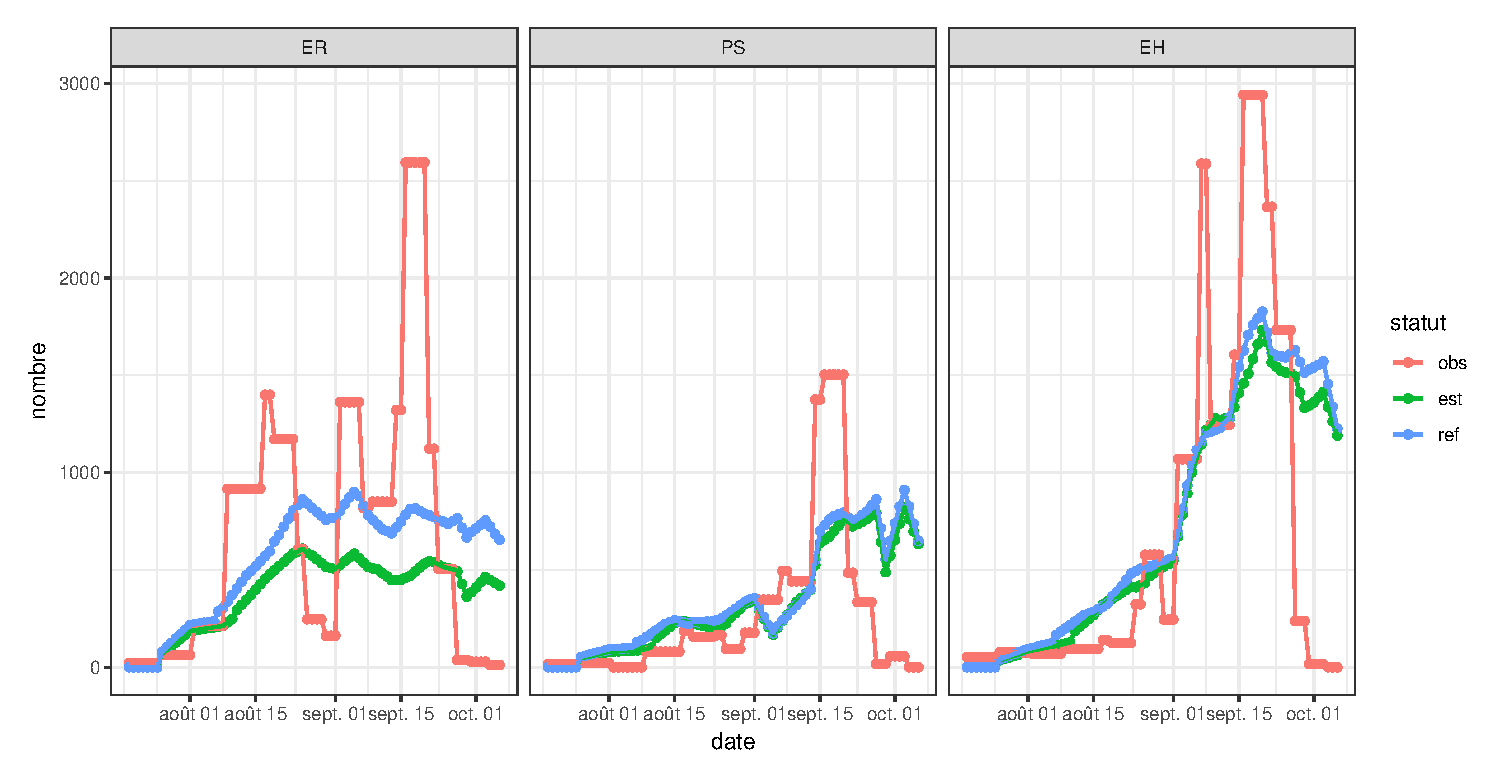
\epsfig{file = plots/pupe_duree9.eps, scale = 0.65}
 \caption{Comparaison des larves observées et estimées. En bleu est visible l'estimation de référence.}
\end{figure}

Les paramètres calibrés sont ici égaux à 

\begin{center}
\begin{tabular}{lllll}
$\gamma$ & $p_m$ & $\mu_{ER}$ & $\mu_{EH}$ & $k$\\
0.038 & 0.7 & 0.6 & 0 & 23.1
\end{tabular}
\end{center}

\newpage
\section{Proba survie paillage synthétique}

Par curiosité, on essaye de fixer $\mu_{PS}$ à 1. On obtient :

\begin{figure}[h]
 \centering
 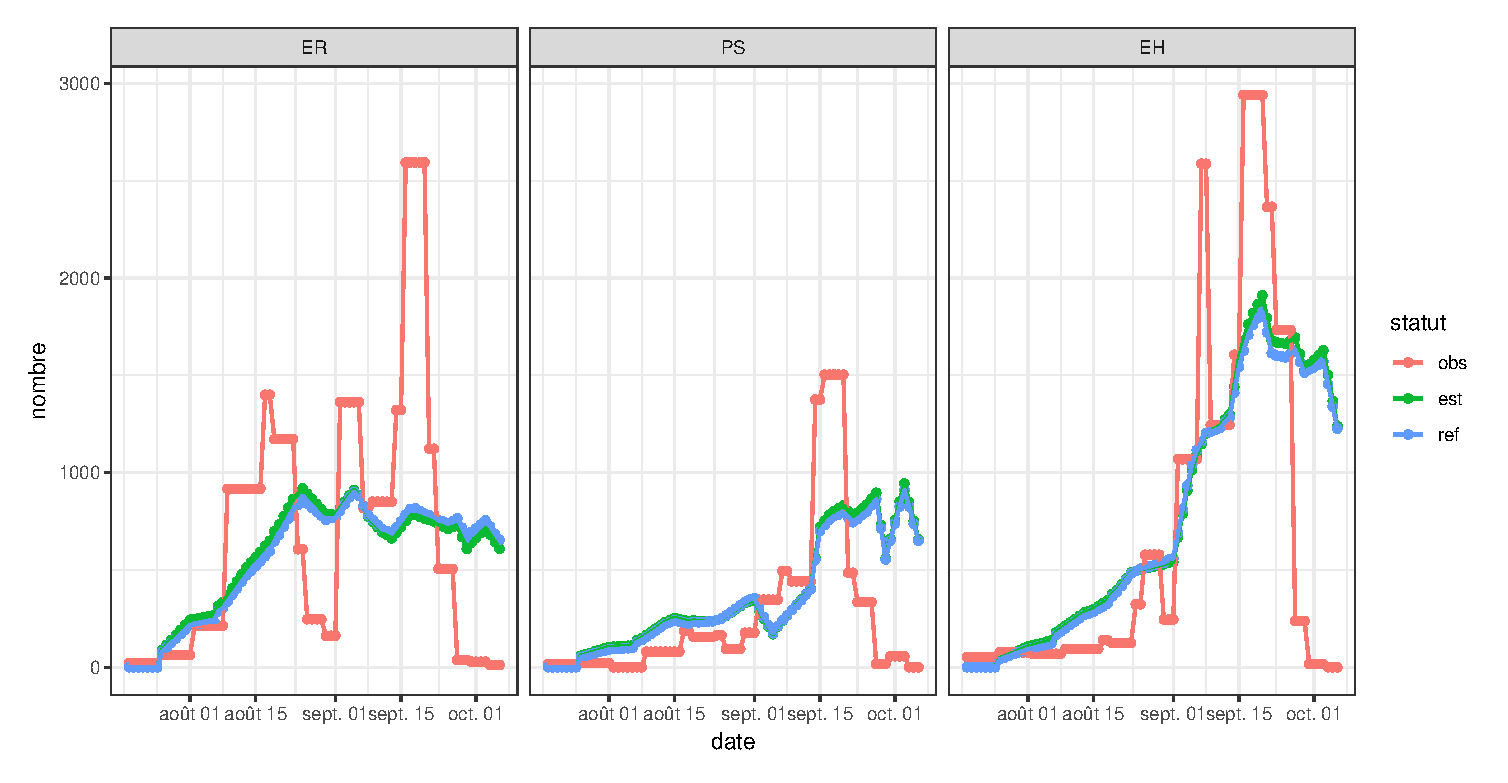
\epsfig{file = plots/muPS1.eps, scale = 0.65}
 \caption{Comparaison des larves observées et estimées. En bleu est visible l'estimation de référence.}
\end{figure}

Les paramètres calibrés sont ici égaux à 

\begin{center}
\begin{tabular}{lllll}
$\gamma$ & $p_m$ & $\mu_{ER}$ & $\mu_{EH}$ & $k$\\
0.043 & 0.57 & 0.50 & 0 & 22.5
\end{tabular}
\end{center}


\newpage
\section{Le sex-ratio}

Avec un $SR = 0$ (\textit{i.e.} uniquement des femelles), on a :
\begin{figure}[h]
 \centering
 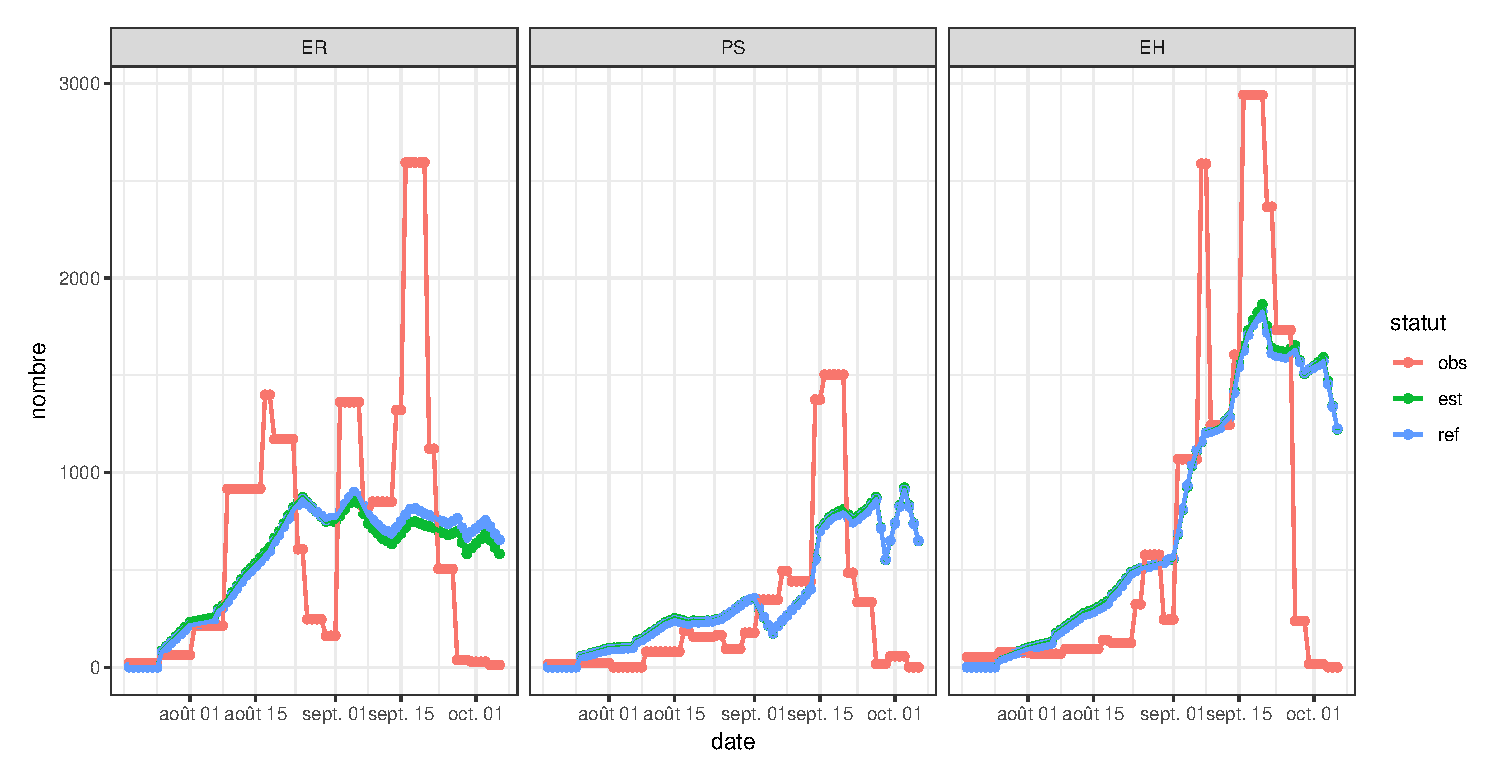
\epsfig{file = plots/sr_0.eps, scale = 0.65}
 \caption{Comparaison des larves observées et estimées. En bleu est visible l'estimation de référence.}
\end{figure}

Les paramètres calibrés sont ici égaux à 

\begin{center}
\begin{tabular}{lllll}
$\gamma$ & $p_m$ & $\mu_{ER}$ & $\mu_{EH}$ & $k$\\
0.041 & 0.62 & 0.27 & 0 & 9.45
\end{tabular}
\end{center}

Avec un $SR = 1$ (\textit{les femelles ne viennent que de l'extérieur}), on a :

\begin{figure}[h]
 \centering
 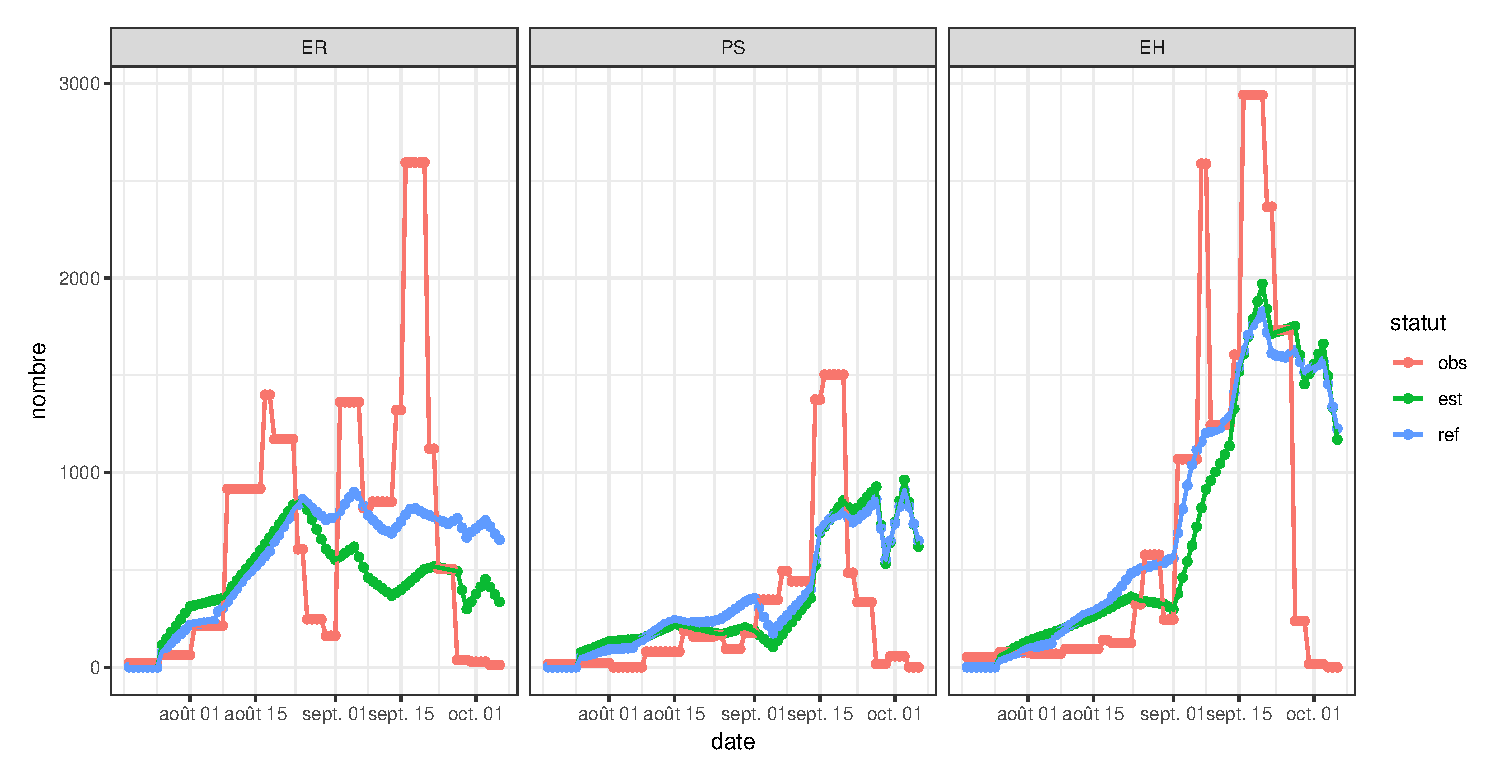
\epsfig{file = plots/sr_1.eps, scale = 0.65}
 \caption{Comparaison des larves observées et estimées. En bleu est visible l'estimation de référence.}
\end{figure}

Les paramètres calibrés sont ici égaux à 

\begin{center}
\begin{tabular}{lllll}
$\gamma$ & $p_m$ & $\mu_{ER}$ & $\mu_{EH}$ & $k$\\
0.054 & 0.64 & 0.25 & 0.1 & 20
\end{tabular}
\end{center}






















 
\end{document}
